\chapter{Конструкторская часть}
В данном разделе будут представлены схемы алгоритмов поиска заданного значения в массиве полным перебором и с помощью двоичного поиска.

\section{Представление алгоритмов}

На вход алгоритмы получают массив $array$ и значение $target$, которое необходимо найти.

На выходе алгоритмы возвращают найденный индекс, а также количество сравнений. В случае отсутствия заданного элемента в массиве алгоритмы, в качестве найденного индекса, возвращают $-1$.

На рисунках \ref{fig:classic_search} --- \ref{fig:bin_search} приведены схемы двух алгоритмов нахождения значения в массиве: использующий полный перебор, использующий бинарный поиск.

\clearpage

\begin{figure}[h]
	\centering
	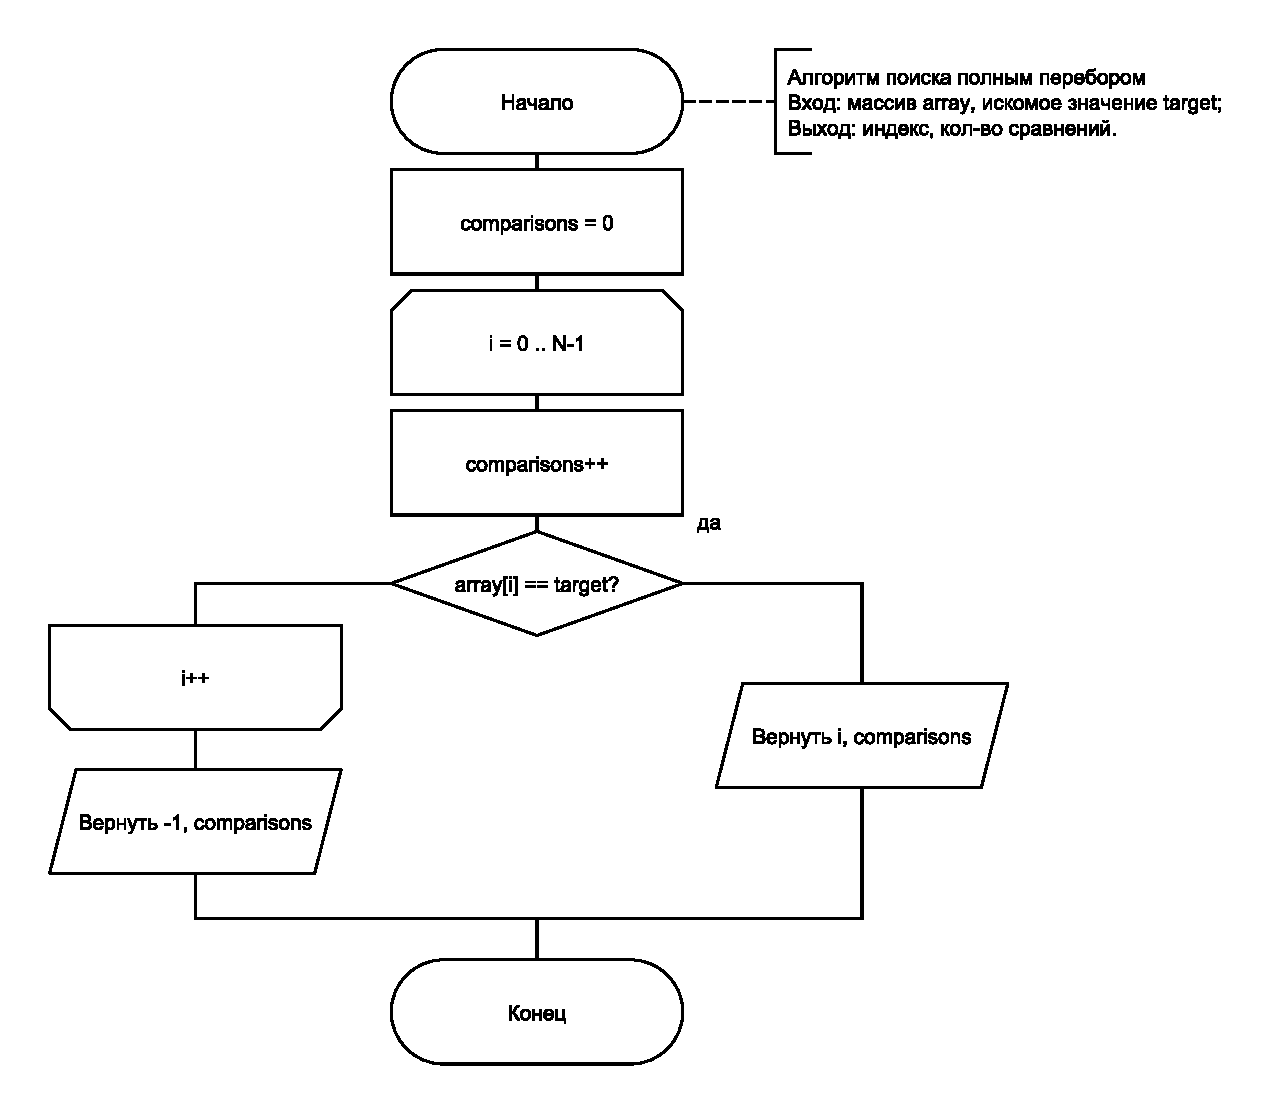
\includegraphics[scale=0.9]{img/fullsearch.eps}
	\caption{Схема алгоритма поиска полным перебором}
	\label{fig:classic_search}
\end{figure}

\clearpage

% \begin{figure}[h]
% 	\centering
% 	\includegraphics[scale=1]{img/vinograd-1-opt.eps}
% 	\label{fig:bin_search-1}
% \end{figure}
\begin{figure}[h]
	\centering
	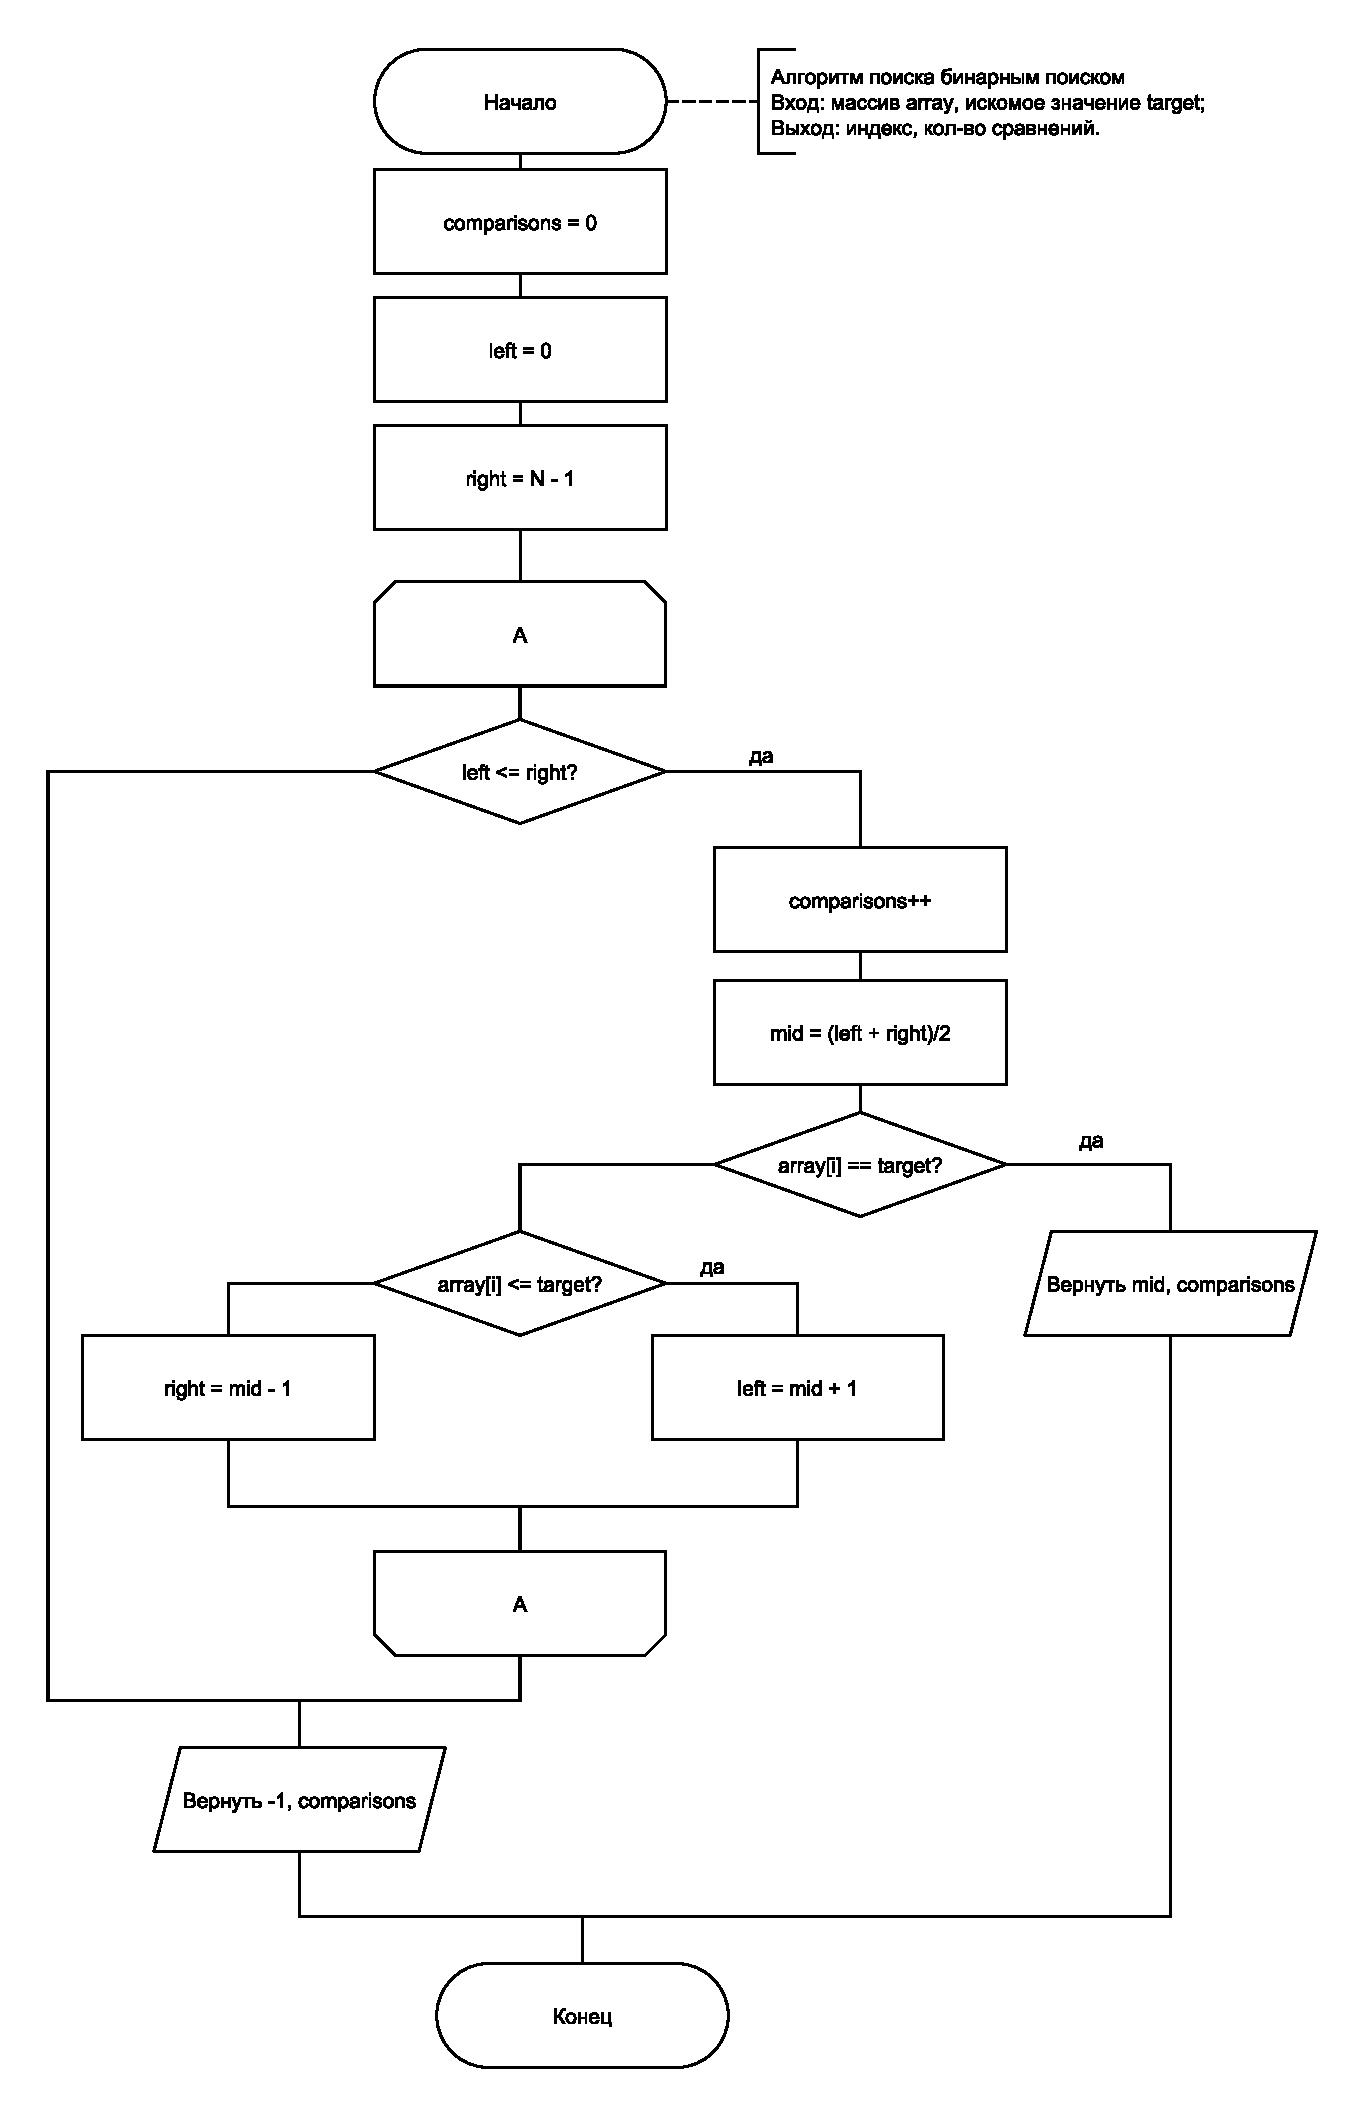
\includegraphics[scale=0.7]{img/binsearch.eps}
	\caption{Схема алгоритма поиска бинарным поиском}
	\label{fig:bin_search}
\end{figure}

\clearpage

\section{Трудоемкость алгоритмов в лучшем и худшем случаях}

Определим трудоемкость в лучшем и худшем случаях для двух алгоритмов.

\subsection{Алгоритм, использующий полный перебор}

В массиве из $N$ элементов $\exists\ N+1$ возможный случай размещения исходного значения $target$ в массиве $array$, включая случай, когда $x \notin array$.

\textbf{Лучший случай:} исходное значение --- первый элемент массива (с индексом $0$). Трудоемкость в лучшем случае составляет $O(1)$.

\textbf{Худший случай:} исходное значение --- последний элемент массива (с индексом $N - 1$). Трудоемкость в худшем случае составляет $O(N)$.

\subsection{Алгоритм, использующий бинарный поиск}

Алгоритм бинарного поиска делит массив пополам на каждом шаге, уменьшая количество элементов, которые нужно проверить.

\textbf{Лучший случай:} искомое значение находится ровно в центре массива на первом шаге. Трудоемкость в лучшем случае составляет \(O(1)\).

\textbf{Худший случай:} искомое значение отсутствует в массиве или расположено на границе одной из половин массива, что требует максимального количества шагов для поиска. Поскольку на каждом шаге массив делится на две части, общее количество шагов для поиска элемента в худшем случае равно \(O(\log N)\).

\vspace{5mm}

\textbf{ВЫВОД}

 В данном разделе были представлены схемы алгоритмов нахождения элемента в словаре.

\clearpage